\documentclass[page number]{beamer}
\usetheme[sectionpage=none,numbering=fraction,progressbar=foot]{metropolis}
\usepackage{etex}
\usepackage{graphicx, booktabs} % For tabulars
\usepackage{pgf,tikz}
\usepackage{ulem}
\usetikzlibrary{arrows}
\usetikzlibrary{positioning,shapes,fit}
\usepackage{multicol}
\usepackage{syntax}
\usepackage{xcolor, color, colortbl}
\usepackage{tikz-qtree}
\usepackage{listings}
\usepackage{mathtools}
\usepackage{amssymb}
\usepackage{amsmath}
\usepackage{pgfgantt}

\makeatletter
\makeatother

%\setcounter{tocdepth}{1} % remove subsection from table of contents

% colors
\definecolor{mDarkRed}{HTML}{6F1616}
\definecolor{mDarkGreen}{HTML}{106235}
\definecolor{mTeal}{HTML}{112233}
\definecolor{mBlack}{HTML}{000000}
\setbeamercolor{normal text}{fg=mTeal}
\setbeamercolor{alerted text}{fg=mDarkRed}
\setbeamercolor{example text}{fg=mDarkGreen}
\setbeamercolor{title separator}{fg=purple,bg=mBlack}
\def\outline{
  \begin{frame}[plain,noframenumbering]
    \frametitle{Outline}
    \tableofcontents[currentsection]
  \end{frame}
}


\begin{document}
\title{Dynamically Scheduled HLS: a Synthesis}

\author[Aur\`ele Barri\`ere]{Aur\`ele Barri\`ere\hfill\textbf{Authors:}\begin{tabular}{c}
    Lana Josipovi\'c\\
    Radhika Ghosal\\
    Paolo Ienne\\
  \end{tabular}}

\date{November 7, 2018}

\def\outline{
  \begin{frame}[plain,noframenumbering]
    \frametitle{Outline}
    \tableofcontents[currentsection]
  \end{frame}
}

\begin{frame}[plain,noframenumbering]
  \vspace{-2cm}
  \maketitle
  \vspace{-4cm}
\end{frame}

\metroset{sectionpage=none}


\metroset{sectionpage=progressbar}
\begin{frame}{Context}
  \begin{block}{FPGAs}
    \begin{itemize}
      \item Great performance
      \item Even more used now (datacenters)
      \item For more general uses
    \end{itemize}
  \end{block}
  \vfill
  \begin{block}{High Level Synthesis}
    Instead of describing directly the circuit, the programmer writes a C program.\\
    HLS generates a circuit.\\
    Less costly to develop.
  \end{block}
\end{frame}

\begin{frame}{Static Scheduling}
  \begin{alertblock}{Static Scheduling}
    The exact cycle where each operation will be executed is decided at synthesis time.
  \end{alertblock}
  \vfill
  \begin{block}{Loop pipelining}
    Each iteration must have the same schedule.
  \end{block}
  \vfill
  \begin{alertblock}{Static scheduling always assume the worst-case scenario}
    When we don't know, we must assume that:
    \begin{itemize}
    \item every branch is taken
    \item every memory access is dependent.
    \end{itemize}
  \end{alertblock}
\end{frame}

\definecolor{blue}{HTML}{74BBC9}

\begin{frame}[fragile]{Static Scheduling: An Example}
  \begin{lstlisting}[language=C]
    for(int i=0; i<100: i++)   {
      d = A[i] * 2;
      if (d >= 0) { s += d; }  } 
  \end{lstlisting}
  \vfill
  \begin{center}
    \texttt{A = [-1, 2, 3, -2, \dots]}
  \end{center}
  \vfill
  \begin{figure}
    %\hspace{-3cm}
    \centering
    \begin{ganttchart}[
        x unit=0.4cm,
        y unit chart=0.4cm,
        canvas/.style={draw=none,fill=none}, % remove canvas borders, etc
        vgrid={*1{draw=black!12}},           % vertical gray lines every unit
        inline,                              % draw bars inline
        group/.style={draw=none,fill=none},  % remove group borders, etc
        bar top shift=0.1,                   % give bar 10% padding top/bottom
        bar height=0.8,                      % bar size 80% of vertical space
        y unit title=0.3cm,                  % crop titles a little smaller
        title/.style={draw=none,fill=none},  % remove title borders, etc
        include title in canvas=false        % no vertical grid in title
      ]{-1}{21}
      
      \ganttgroup[inline=false]{$i=1$}{0}{1}
      \ganttbar[bar/.style={fill=yellow}]{\texttt{Rd}}{0}{0}
      \ganttbar[bar/.style={fill=blue}]{\texttt{*}}{1}{4} 
      \ganttbar[bar/.style={fill=yellow}]{\texttt{>=}}{5}{5}
      \ganttbar[bar/.style={fill=red}]{\texttt{+}}{6}{9}\\
      
      \ganttgroup[inline=false]{$i=2$}{0}{1}
      \ganttbar[bar/.style={fill=yellow}]{\texttt{Rd}}{4}{4}
      \ganttbar[bar/.style={fill=blue}]{\texttt{*}}{5}{8} 
      \ganttbar[bar/.style={fill=yellow}]{\texttt{>=}}{9}{9}
      \ganttbar[bar/.style={fill=blue}]{\texttt{+}}{10}{13}\\
      
      \ganttgroup[inline=false]{$i=3$}{0}{1}
      \ganttbar[bar/.style={fill=yellow}]{\texttt{Rd}}{8}{8}
      \ganttbar[bar/.style={fill=blue}]{\texttt{*}}{9}{12} 
      \ganttbar[bar/.style={fill=yellow}]{\texttt{>=}}{13}{13}
      \ganttbar[bar/.style={fill=blue}]{\texttt{+}}{14}{17}\\
      
      \ganttgroup[inline=false]{$i=4$}{0}{1}
      \ganttbar[bar/.style={fill=yellow}]{\texttt{Rd}}{12}{12}
      \ganttbar[bar/.style={fill=blue}]{\texttt{*}}{13}{16} 
      \ganttbar[bar/.style={fill=yellow}]{\texttt{>=}}{17}{17}
      \ganttbar[bar/.style={fill=red}]{\texttt{+}}{18}{21}
      
      
    \end{ganttchart}
    %\caption{Static scheduling with loop pipelining. Red operations are not actually used}
    %\label{fig:static_schedule}
  \end{figure}
\end{frame}

\begin{frame}{Why dynamic scheduling?}
  \begin{block}{Dynamic Scheduling}
    Choose dynamically when to execute each operation.\\
    Don't schedule unused operations.\\
    Execute operations as soon as possible.
  \end{block}
  \vfill
  \begin{figure}
    \centering
    \begin{ganttchart}[
	x unit=0.4cm,
	y unit chart=0.4cm,
	canvas/.style={draw=none,fill=none}, % remove canvas borders, etc
	vgrid={*1{draw=black!12}},           % vertical gray lines every unit
	inline,                              % draw bars inline
	group/.style={draw=none,fill=none},  % remove group borders, etc
	bar top shift=0.1,                   % give bar 10% padding top/bottom
	bar height=0.8,                      % bar size 80% of vertical space
	y unit title=0.3cm,                  % crop titles a little smaller
	title/.style={draw=none,fill=none},  % remove title borders, etc
	include title in canvas=false        % no vertical grid in title
      ]{-1}{21}
      
      \ganttgroup[inline=false]{$i=1$}{0}{1}
      \ganttbar[bar/.style={fill=yellow}]{\texttt{Rd}}{0}{0}
      \ganttbar[bar/.style={fill=blue}]{\texttt{*}}{1}{4} 
      \ganttbar[bar/.style={fill=yellow}]{\texttt{>=}}{5}{5}\\
      %\ganttbar[bar/.style={fill=red}]{\texttt{+}}{6}{9}\\
      
      \ganttgroup[inline=false]{$i=2$}{0}{1}
      \ganttbar[bar/.style={fill=yellow}]{\texttt{Rd}}{1}{1}
      \ganttbar[bar/.style={fill=blue}]{\texttt{*}}{2}{5} 
      \ganttbar[bar/.style={fill=yellow}]{\texttt{>=}}{6}{6}
      \ganttbar[bar/.style={fill=blue}]{\texttt{+}}{7}{10}\\
      
      \ganttgroup[inline=false]{$i=3$}{0}{1}
      \ganttbar[bar/.style={fill=yellow}]{\texttt{Rd}}{2}{2}
      \ganttbar[bar/.style={fill=blue}]{\texttt{*}}{3}{6} 
      \ganttbar[bar/.style={fill=yellow}]{\texttt{>=}}{7}{7}
      \ganttbar[bar/.style={fill=blue}]{\texttt{+}}{11}{14}\\
      
      \ganttgroup[inline=false]{$i=4$}{0}{1}
      \ganttbar[bar/.style={fill=yellow}]{\texttt{Rd}}{3}{3}
      \ganttbar[bar/.style={fill=blue}]{\texttt{*}}{4}{7} 
      \ganttbar[bar/.style={fill=yellow}]{\texttt{>=}}{8}{8}
      %\ganttbar[bar/.style={fill=red}]{\texttt{+}}{18}{21}
    \end{ganttchart}
  \end{figure}
\end{frame}

\begin{frame}{Elastic Circuits}
  Introduced by Cortadella, Kishinevsky and Grundmann in 2006.
  \vfill
  \begin{block}{Elastic circuits}
    \begin{itemize}
    \item Originally, for latency-insensitive circuits.
    \item Handshake protocol.
    \end{itemize}
  \end{block}
  \vfill
  \begin{block}{The SELF protocol}
    Each block has a \textit{Valid} and a \textit{Stop} signal.
  \end{block}
      
\end{frame}

\begin{frame}{Elastic Circuits: An Example}
  \begin{columns}
    \begin{column}{0.4\textwidth}
      \scriptsize
\texttt{for(int i=0; i<100; i++)   \{}\\
\texttt{d = A[i] * 2;}\\
\texttt{if (d >= 0) \{ s += d; \}  \} }
      \normalsize    
    \end{column}
    \begin{column}{0.6\textwidth}  %%<--- here
      \begin{center}
        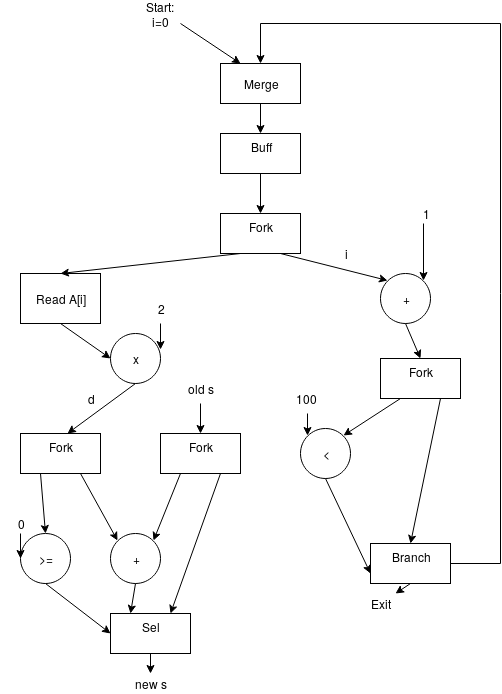
\includegraphics[scale=0.3]{circuit.png}
      \end{center}
    \end{column}
  \end{columns}
\end{frame}

\begin{frame}{Synthesizing Elastic Circuits}
  \begin{block}{Basic Blocks}
    Block without linear control-flow.\\
    Extracted from the CFG.
  \end{block}
  \vfill
  \begin{block}{Connecting Basic Blocks}
    Avoid deadlocks.\\
    Coupling dataflow with control-flow.
    TODO
  \end{block}
      
\end{frame}

\begin{frame}{Memory Accesses}
  \begin{alertblock}{Out-of-order memory accesses}
  \end{alertblock}
  \vfill
  \begin{exampleblock}{The Solution: a Load-Store Queue}
    Comes from dynamically scheduled processors.\\
    Give it the original order of memory accesses.
  \end{exampleblock}
  \vfill
  \begin{block}{Lazy Forks}
    Wait for both receiving blocks to be ready.
  \end{block}
    
\end{frame}

\begin{frame}{Improvements}
  \begin{block}{Adding Elastic Buffers}
    Reduce the crtical path's length.\\
    At least one on each cycle.\\
    No buffers in front of the LSQ.
  \end{block}
  \vfill
  \begin{block}{Adding Elastic FIFOs}
    When some path takes more time, allows token accumulation without stopping the whole circuit.
  \end{block}
  \vfill
  TODO:Figure
\end{frame}

\begin{frame}{Implementation}
  TODO:schema
\end{frame}

\begin{frame}{Benchmark}
  \begin{block}{Histogram}
    Goes through an array and increases histogram bars.\\ Independent memory accesses?
  \end{block}
  \vfill
  \begin{block}{Matrix Power}
  \end{block}
  \vfill
  \begin{block}{2 loops}
    One is optimized in order to use less circuit during synthesis.
  \end{block}
  \vfill
  \begin{alertblock}{FIR Filter}
    Every access is statically known to be independent.\\
    Static shceduling exploits all parallelism.\\
    Used to estimate the overhead of dynamic scheduling.
  \end{alertblock}
\end{frame}

\def\g#1{{\textbf{\color{mDarkGreen}#1}}}
\def\r#1{{\textbf{\color{mDarkRed}#1}}}
\begin{frame}{Results against Static HLS}
  \tiny
  \hspace*{-8pt}\makebox[\linewidth][c]{%
    \begin{tabular}{l c c c c c c}
      \textbf{Benchmark} & \textbf{Execution Time STAT} & \textbf{Execution Time DYN} & \textbf{Slices STAT} & \textbf{Slices DYN} & \textbf{II STAT} & \textbf{II DYN}\\
      \texttt{Histogram} & 36.3 us & \g{13.3} us & 130 & \r{1101} & 11 & \g{2.3}\\
      \texttt{Matrix power} & 20.7 us & \g{9.6} us & 219 & \r{1465} & 16 & \g{4.2}\\
      \texttt{Loop 1} & 25.3 us & \g{6.2} us & 161 & \r{289} & 9 & \g{1.3}\\
      \texttt{Loop 2} & 17.1 us & \g{5.7} us & 187 & \r{240} & 5 & \g{1.2}\\
      \texttt{FIR filter} & 3.3 us & \r{4.4} us & 62 & \r{127} & 1 & 1
    \end{tabular}%
  }
  \vfill
  \normalsize
  \begin{exampleblock}{Better Execution Time}
    The overhead is not that significant compared to the gain.
  \end{exampleblock}
  \vfill
  \begin{alertblock}{More circuit complexity}
  \end{alertblock}
    
\end{frame}

\begin{frame}{Results against Dynamic Techniques}
  \begin{block}{Huang}
    Elastic Circuits for CGRAs.\\
    No pipeline.
  \end{block}
  \vfill
  \begin{block}{Cash}
    Generate asynchronous circuits from C code.\\
    Conservative memory handling.
  \end{block}
  \vfill
  \tiny
  \hspace*{-8pt}\makebox[\linewidth][c]{%
    \begin{tabular}{l c c c c c c}
      \textbf{Benchmark} & \textbf{Time HUANG} & \textbf{Time CASH} & \textbf{Time DYN} & \textbf{Slices HUANG} & \textbf{Slices CASH} & \textbf{Slices DYN}\\
      \texttt{Histogram} & 58.9 us & 21.2 us & \g{13.3} us & 134 & 1083 & \r{1101}\\
      \texttt{Matrix power} & 26.2 us & 11.9 us & \g{8.6} us & 204 & 1445 & \r{1465}
    \end{tabular}%
  }
\end{frame}

\begin{frame}{Conclusion}
  \begin{alertblock}{Limits of static scheduling}
  \end{alertblock}
  \vfill
  \begin{exampleblock}{Using Elastic Circuits for Dynamic HLS}
    General, automatic synthesis of elastic circuits.
  \end{exampleblock}
  \vfill
  \begin{exampleblock}{Implementation and Benchmarks}
    Promising Results.
  \end{exampleblock}
  \vfill
  \begin{block}{Tradeoff}
    Performance and Circuit Complexity.\\
    Better for non-regular programs.
  \end{block}
\end{frame}

\begin{frame}{Further Work}
  \begin{block}{Optimizations}
    \begin{itemize}
    \item Optimize circuit complexity.
    \item Optimize buffer placement.
    \item Others?
    \end{itemize}
  \end{block}
  \vfill
  \begin{block}{Speculative Execution}
    It has been showed that elastic circuit can be accomodated to fit speculaive execution.
  \end{block}
\end{frame}

\begin{frame}{Overview}
  Published in FPGA 18.\\
  4 citations.\\
  Good methodology.\\
  Semimanual steps?
  \vfill
  TODO
  
\end{frame}
    

\end{document}
